% !TeX root = ../main.tex
\subsection{Data applications}
\label{sec:applications}

We apply the individual sampler of Section~\ref{subsec:individual} to two real data sets, each with a frequentist benchmark. The first is one day of readings from a low-cost air-quality sensor, aggregated to $n = 8{,}640$ observations, where the target is a low quantile of the series that serves as its baseline. The second is the height of 4{,}817 boys and 5{,}190 girls aged 0 to 22 years from the Fifth Dutch Growth Study, where the target is a family of five quantile curves in age.

\subsubsection{Air-quality sensor data}
\label{sec:app:spod}

The first application is the fenceline monitoring problem for which \citet{brantley2020baseline} developed quantile trend filtering. The U.S.\ Environmental Protection Agency places low-cost SPod sensors on the perimeter of industrial facilities to detect fugitive emissions of volatile organic compounds. Each sensor records, once per second, the signal of a photoionization detector (PID) in uncalibrated counts. Emission plumes produce one-sided spikes lasting seconds to a few minutes, on a baseline that drifts over hours with temperature, humidity, and lamp condition. The baseline is therefore a low conditional quantile of the series, and it must be removed before events can be flagged or compared across sensors.

We analyze one day of data, June 15, 2018, from sensor \texttt{d} of the two collocated SPods in the EPA Rubbertown data set accompanying \citet{brantley2020baseline}. The day has $86{,}179$ usable 1-Hz readings; the other seconds are absent or, for $30$ consecutive seconds, recorded as not available. The readings are aggregated into 10-second means of the available readings, so that $n = 8{,}640$ ($19$ of the $8{,}640$ blocks, which contain no reading, are linearly interpolated). The aggregation attenuates the strong serial correlation of the 1-Hz noise, which the ALD working likelihood does not model.

We estimate the baseline at the three levels $\tau \in \{0.01, 0.05, 0.10\}$ with $k = 2$. Each level is fitted separately by the individual sampler on the standardized series, with the sampler and settings of Section~\ref{sec:air_simulation}. The series has the structure of that simulation, short one-sided plumes on a slowly varying baseline, and by the argument given there we use the same prior, $\lambda \sim \mathrm{Gamma}(n, 10^{-2})$ with $n = 8{,}640$. At each level we run two chains of $30{,}000$ sweeps with a burn-in of $10{,}000$, pool every $30$th retained draw of both, and report the pointwise posterior median, transformed back to counts. Under this prior the trend mixes slowly (Appendix~\ref{app:pmala:interior}), so the curves are reported as point estimates, without intervals.

As the frequentist benchmark we use the ADMM solver of the \texttt{detrendr} package of \citet{brantley2020baseline}. Its penalty is selected by extended BIC over the grid $\lambda \in \exp\{-2, \dots, 12\}$. The criterion selects $\lambda = 54.6$ at $\tau = 0.01$ and $\lambda = 1096.6$ at $\tau \in \{0.05, 0.10\}$. Following \citet{brantley2020baseline}, we detect events by a threshold rule on the detrended series $\by - \widehat{\theta}$: a point is classified as signal when it exceeds the empirical 90th, 95th, or 99th percentile of the detrended data. The rule requires no absolute calibration of the counts.

\begin{figure}[tbp]
\centering
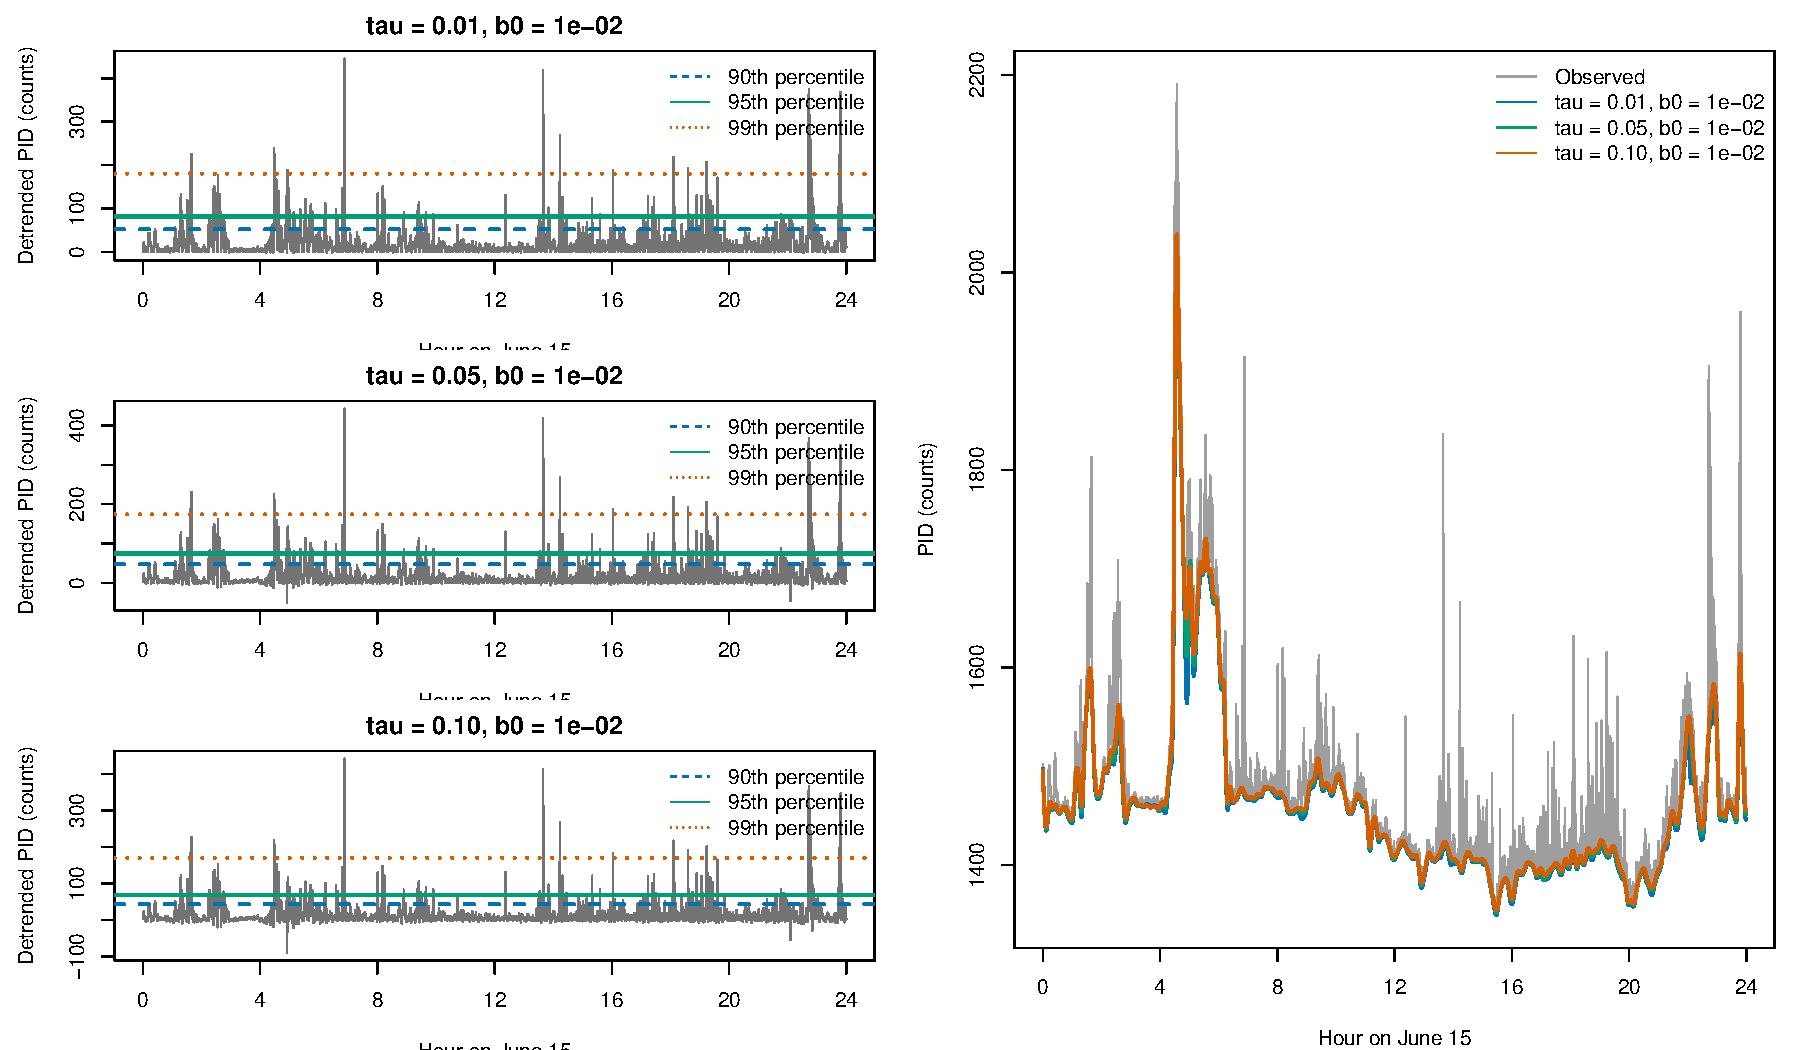
\includegraphics[width=\textwidth]{figures/spod_pmala_e18}
\caption{Air-quality data: Bayesian-PMALA fits with $k = 2$ and $\lambda \sim \mathrm{Gamma}(n, 10^{-2})$ on the 10-second means ($n = 8{,}640$) of SPod \texttt{d}, June 15, 2018. Left: detrended series $\by - \widehat{\theta}$, one panel per quantile level, with the 90th (dashed), 95th (solid), and 99th (dotted) empirical percentiles of the detrended data, the thresholds used to classify emission events. Right: baseline trends at $\tau \in \{0.01, 0.05, 0.10\}$, with the observed PID series in gray. Curves are pointwise posterior medians of two pooled chains.}
\label{fig:spod_pmala}
\end{figure}

The right panel of Figure~\ref{fig:spod_pmala} shows the three fitted baselines for Bayesian-PMALA; the ADMM fits and the detrended series they produce are in Appendix~\ref{app:spod_admm}. Both methods place most of the large excursion between 04:30 and 06:00 in the baseline, follow the slow decline through the afternoon, and leave the short plume spikes above the fit. The fraction of observations below the fitted curve is $0.009$, $0.059$, and $0.116$ at $\tau = 0.01, 0.05, 0.10$ for Bayesian-PMALA, against $0.000$, $0.043$, and $0.092$ for ADMM.

The three levels are fitted separately, so the curves are not constrained to be ordered, and they lie close together: the median distance between adjacent curves is about $1.5$ counts. At $1{,}097$ of the $8{,}640$ time points at least one adjacent pair is in the wrong order (the $0.01$ curve is above the $0.05$ curve at $812$ points, and the $0.05$ curve above the $0.10$ curve at $427$), by at most $6.3$ counts. The ADMM curves also cross: extended BIC selects a penalty twenty times smaller at $\tau = 0.01$ than at the other two levels, and the resulting curve bends upward into the plume near 05:00 and crosses the other two. The joint sampler of Section~\ref{subsec:joint}, which excludes crossings, was not run on these data.

The left panels of Figure~\ref{fig:spod_pmala} show the detrended series with the three detection thresholds, and Figure~\ref{fig:spod_detrended_admm} shows the ADMM counterpart. With the $\tau = 0.05$ baseline removed, the 95\% threshold is $74$ counts for Bayesian-PMALA and $92$ for ADMM, whereas the largest plume exceeds $400$ counts. The events of interest are therefore separated from the noise under either baseline.

Each chain of $30{,}000$ sweeps at $n = 8{,}640$ took between $37$ and $49$ minutes on one core of a Linux compute cluster. The ADMM fit with its grid search took roughly four minutes; it was not timed on the same machine, so the two times are not directly comparable.

\subsubsection{Growth centiles for Dutch children}
\label{sec:app:growth}

The second application is the growth chart: a child's height is read against the population centiles at the same age, so the chart is a family of quantile curves indexed by age. We use the Fifth Dutch Growth Study \citep{schonbeck2013tallest}, a nationwide cross-sectional sample collected in 2009 and distributed with the \texttt{mice} package \citep{vanbuuren2011mice}. After removing records without a height measurement, the data contain 4{,}817 boys and 5{,}190 girls aged 0 to 22 years, each measured once. Boys and girls are analyzed separately.

In contrast with the simulation designs, many children share a covariate value. We round age to the nearest tenth of a year, which gives a grid of $G = 220$ equally spaced ages for boys and $G = 221$ for girls, and index the trend $\theta \in \R^{G}$ by grid point. The ALD likelihood sums the check loss over all children at a grid point, so that each $\theta_g$ is informed by every height recorded at grid point $g$. In the augmented sampler each child keeps its own latent variable $z_i$, and the scale update \eqref{eq:sigmaupdate} runs over all children. In the trend target \eqref{eq:Utheta}, the Gaussian terms of the children at grid point $g$ combine into a single term in $\theta_g$, whose weight is the sum of their $w_i$ and whose center is the $w$-weighted mean of their $r_i$. Because the grid is equally spaced, the difference operator is the usual one, and the samplers apply without other changes.

We use $k = 2$ and $\lambda \sim \mathrm{Gamma}(1, \sqrt{G})$. Each level $\tau \in \{0.1, 0.3, 0.5, 0.7, 0.9\}$ is fitted by an independent run of 6{,}000 sweeps with 1{,}000 burn-in, and we report the posterior mean. This rate differs from those of the simulations, which have one observation per design point, because with some twenty children per grid point the likelihood is much more concentrated.

As a benchmark we fit the LMS method \citep{cole1992smoothing}, the standard tool for growth references. At each age, height is assumed to follow a Box--Cox Cole--Green distribution whose median, coefficient of variation, and Box--Cox power are smooth functions of age. All centiles are read off this one fitted distribution, so they cannot cross; the method assumes a parametric shape at every age. We use the \texttt{lms} function of the \texttt{gamlss} package \citep{rigby2005generalized}.

Figure~\ref{fig:growth_boys} shows the five fitted quantile curves for boys. The curves follow the fast growth in infancy, the near-linear childhood phase, the pubertal spurt, and the adult plateau, and they fan out with age as the height distribution widens. In-sample calibration is close to nominal: the fraction of boys below the fitted curve is $0.098$, $0.300$, $0.498$, $0.699$, and $0.903$ at $\tau = 0.1, 0.3, 0.5, 0.7, 0.9$.

The five fits are independent, so non-crossing is not enforced. The posterior-mean curves for girls do not cross. Those for boys cross in one of $880$ adjacent comparisons: at age $0.1$ years the $0.5$ curve lies $0.6$~cm above the $0.7$ curve.

The girls' fit and the LMS centiles for both sexes are in Appendix~\ref{app:growth} (Figures~\ref{fig:growth_girls}--\ref{fig:growth_lms_girls}). The two methods agree between about one and eighteen years of age and differ at the ends of the age range, where few children are observed. The LMS centiles follow the local data more closely. The trend filtering curves extrapolate the piecewise-quadratic trend: they lie slightly above the newborn measurements and bend at the oldest ages.

\begin{figure}[htbp]
\centering
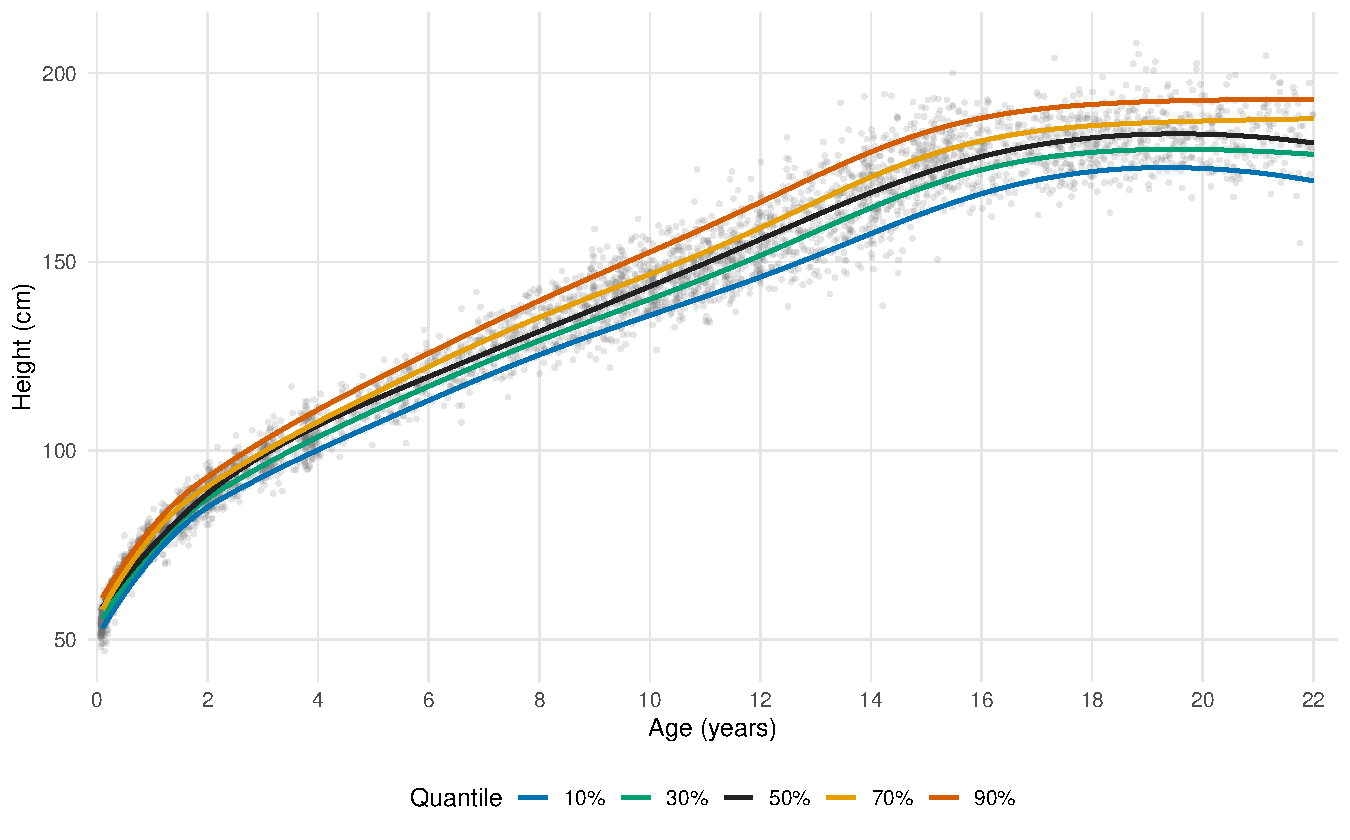
\includegraphics[width=0.75\textwidth]{figures/growth_pmala_boys}
\caption{Bayesian-PMALA fits for the height of 4{,}817 Dutch boys from the Fifth Dutch Growth Study \citep{schonbeck2013tallest} at $\tau \in \{0.1, 0.3, 0.5, 0.7, 0.9\}$, $k = 2$. Curves are posterior means on the 0.1-year age grid; gray circles are the individual measurements. Each level is fitted independently.}
\label{fig:growth_boys}
\end{figure}
